

The EIC will be a large international project with many researchers and stakeholders spread throughout the globe. While the accelerator and detectors are necessarily placed at a single locale, the computing need not be and can better reflect the geographic diversity of the collaborations involved in EIC research. In the modern age, high speed network connectivity has become very robust. In the time frame of the EIC ($\sim 2030$) we can expect even more reliable and even faster networks. This will make transporting data on the scale the EIC is expected to produce fairly routine. To give specific numbers, BNL has a 400Gbps connection to the ESnet backbone in 2021. ECCE is currently estimated to produce 100Gbps of raw data once it is in full production sometime around 2030. Network bandwidths have shown steady growth of about 50\% per year over the past few decades\cite{nielsensLaw2019}. Thus, over the next 8 years we can expect existing bandwidths to grow by roughly a factor of 25. Even a conservative estimate that the BNL external connection bandwidth grows by only a factor of 10 means the entire ECCE raw data volume can be streamed out using only a few percent of the total available bandwidth.

This section will briefly describe how a federated computing model for the EIC might look, how it will be used to process the raw data, and how it will also be used to process the large amounts of simulation needed for the program.

%-------------------------------------------------------------------
\subsection{Federated computing}

EIC data processing will employ a federated computing model where multiple facilities will be used. A similar strategy has been successfully deployed by the LHC in the form of the Worldwide LHC Computing Grid (WLCG) or simply \emph{the Grid}\cite{SHIERS2007219}. The benefits of distributing the computing across multiple sites include:

\begin{itemize}
    \item Each site only needs to handle a fraction of data
    \item EIC computing becomes a smaller fraction of each compute farm
    \item One site having diminished capacity temporarily can easily be absorbed by others without reconfiguration
\end{itemize}

Generally speaking, diversifying helps to mitigate certain risks. 

The WLCG model of the LHC is based on multiple \emph{Tiers}, structured in a pyramid type fashion. The topmost tier (\emph{Tier 0})represents the LHC/CERN where the data is produced and all data is stored. It also supplies around 20\% of the total computing resource and does the initial reconstruction of the data before distributing it to the Tier 1 sites\cite{WLCG_Tiers_website}. The Tier 1 sites perform large scale reprocessing of the data and distribution to the Tier 2 sites. The Tier 2 sites do more specialized analysis and simulations while the Tier 3 sites are end users. Each tier in the system only communicates with tiers directly above or below it in the hierarchy.

For the EIC one may consider an alternative model in which the data producer (the experiments of the EIC) and the BNL compute facility (e.g. SDCC) are independent. This allows computing at BNL to become part of a pool of facilities that handle the computing as a federated resource. Figure \ref{fig:federated_offsite_butterfly} illustrates such a model referred to here as a ``\emph{Butterfly}'' model due to the rough shape of the figure. In this model, both compute and storage are distributed with the storage being focused in the Echelon 1 sites. This means access to the data by the end users will be done by connecting Echelon 3 sites directly to Echelon 1 sites. The Echelon 1 sites will themselves provide significant compute capability, but may also farm out large campaigns to Echelon 2 sites. In the simulation campaigns performed for the ECCE proposal, the model shown in Fig.~\ref{fig:federated_offsite_butterfly} was successfully implemented for simulated data production.

\begin{figure}[hbt!]
 \begin{center}
   \raisebox{0.5mm}{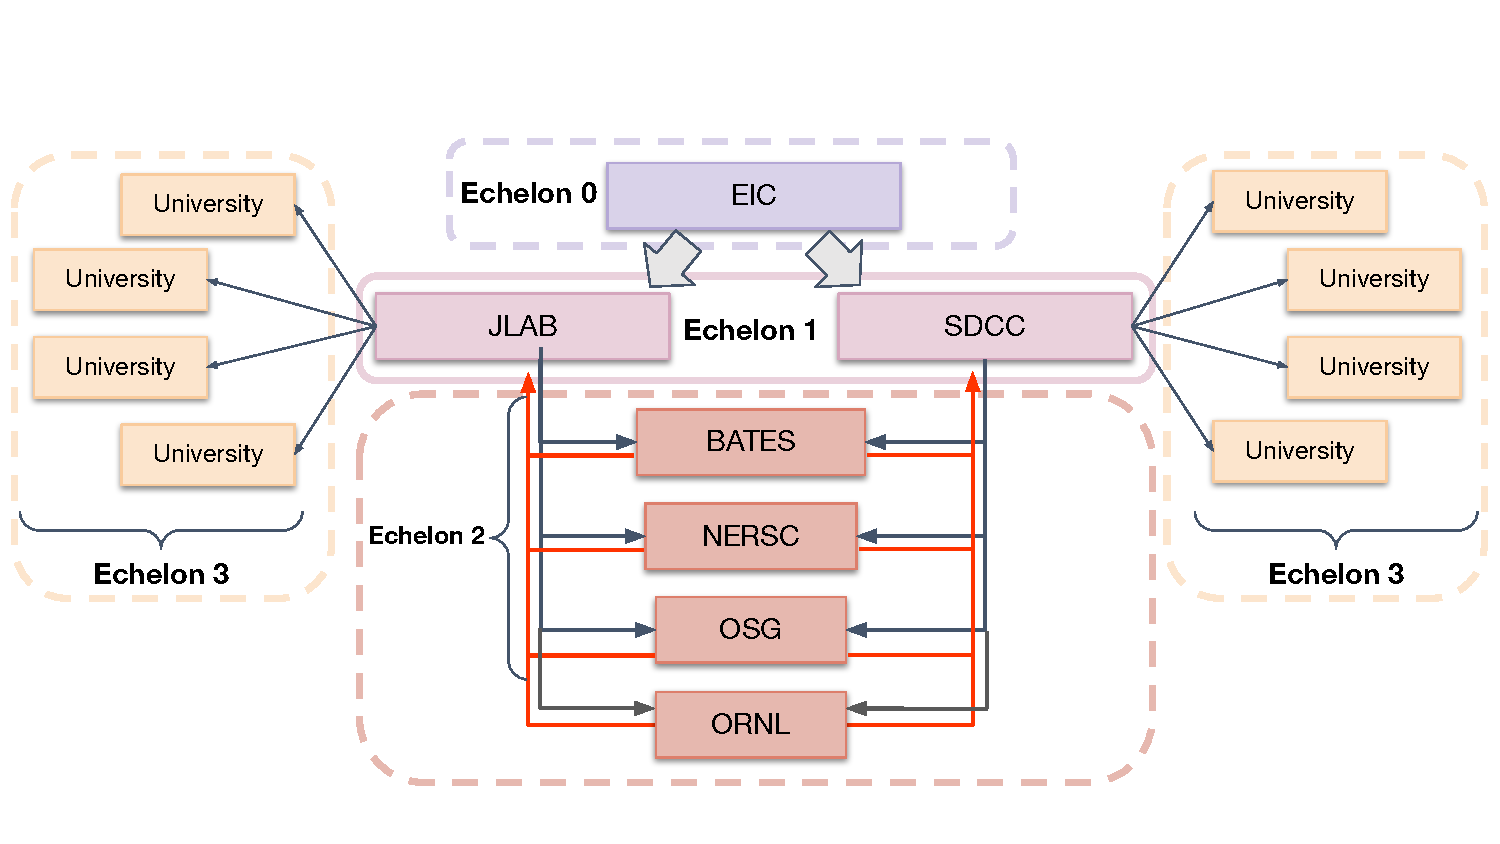
\includegraphics[clip, width=0.99\linewidth]{figs/computing_figure_federated_offsite_butterfly.pdf}}
  \caption[Federated Computing Butterfly model.]{\label{fig:federated_offsite_butterfly} Butterfly model of federated offsite computing. In this model, nearly all storage is contained in echelon 1 while large portions of the raw data processing is delegated to multiple HTC/HPC facilities. The named facilities in this graphic are merely examples and do not represent commitments or final plans.}
 \end{center}
\end{figure}

%-------------------------------------------------------------------
\subsection{Raw data compute}
Processing of EIC data will occur over multiple sites which will include HTC facilities at both BNL and JLab and possibly others. The plan calls for processing the raw data into reconstructed objects such as tracks, jets, and calorimeter clusters within 2-3 weeks of acquisition. The bulk of the few week latency will be due to the time it takes to calibrate the data so that reconstruction may occur. Figure \ref{fig:federated_offsite_example} illustrates how such a scheme could work. The raw data read from the streaming DAQ system will need to be reduced over multiple filtering and compression stages to a rate that is reasonable to transport offsite from BNL using its external network connection. Table \ref{tab:reduction_factors} lists the stages and with in-going and out-going rates and their respective reduction factors. Potential technologies that could be applied at each stage are also listed.

The DOE lab systems are connected via the ESNet unclassified network for scientific research~\cite{ESNet}. As of 2021, BNL has a 400Gbps connection to ESNet and JLab has dual 10Gbps connections. In 2022 or 2023, JLab is anticipated to increase its bandwidth to at least 100Gbps. When the EIC begins collecting data around 2030, one may expect a 1Tbps bandwidth between the two labs. This is an order of magnitude higher than the anticipated raw data rate after filtering from the ECCE detector. Thus, transfer of the entire raw data set offsite from BNL in 2030 seems reasonable.


\begin{figure}[hbt!]
 \begin{center}
   \raisebox{0.5mm}{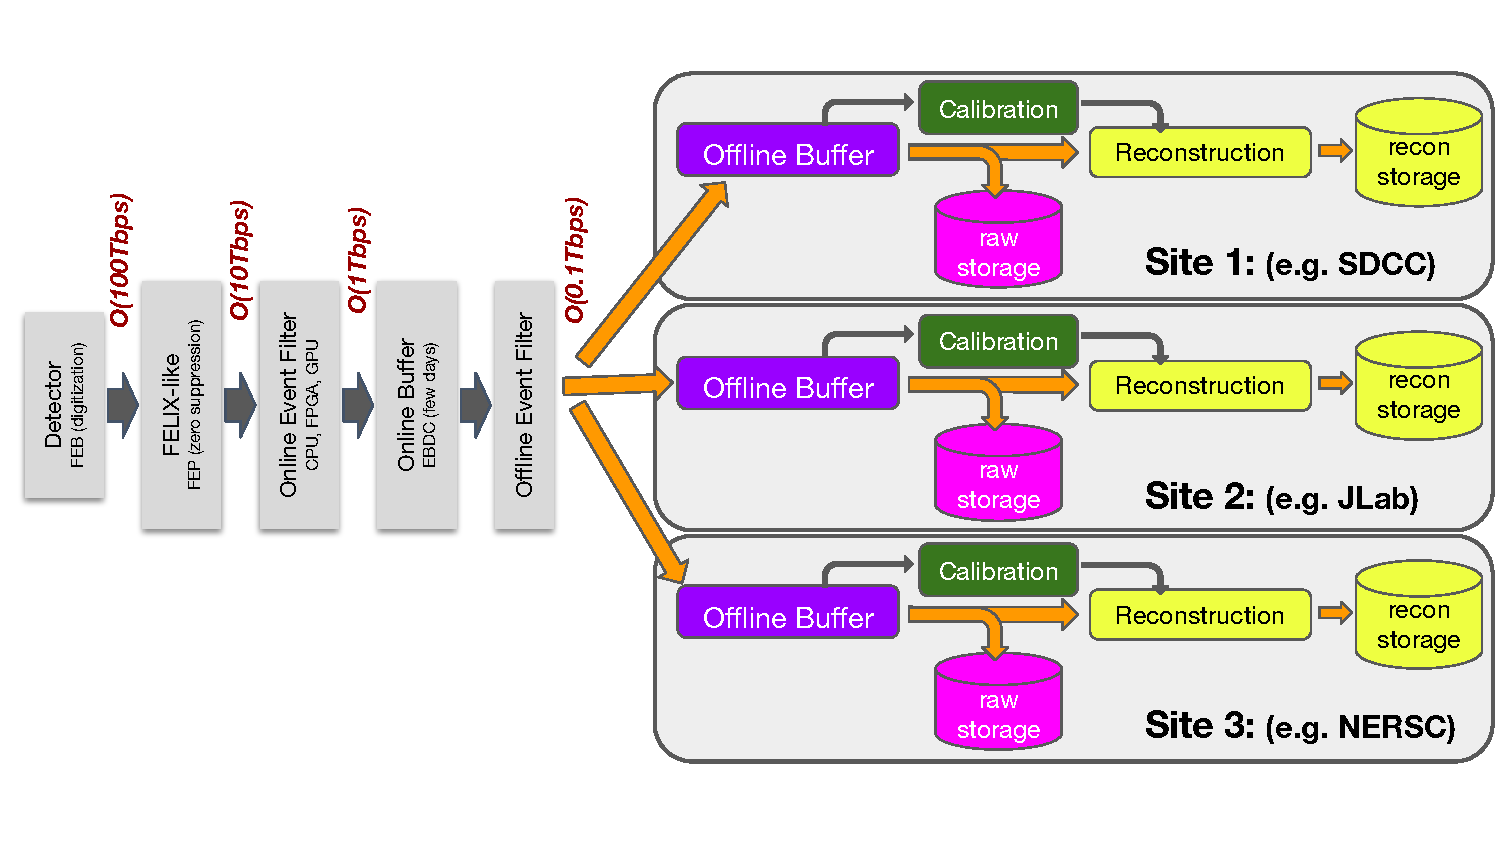
\includegraphics[clip, width=0.99\linewidth]{figs/figure_federated_offsite_example.pdf}}
  \caption[Example of federated processing of data in near real-time using multiple sites.]{\label{fig:federated_offsite_example} Data flow from detector to reconstructed object files (left to right). This diagram illustrates how raw data may be distributed to multiple sites in near-real time. On the left side of the plot, multiple filter and buffering stages are used to reduce the data rate. On the right, the data is distributed to multiple facilities.
  Each facility would store a portion of the raw data. It would also need to keep the data live (e.g. on disk) long enough for it to be calibrated and then processed by the reconstruction software.}
 \end{center}
\end{figure}

\begin{table*}[ht]
    \centering
    \begin{tabular}{p{4cm}|c|c|c}
        \hline
        Stage                        & Input/Output    & Reduction Factor & Technology options \\
        \hline
        \hline
        Compute Interface (e.g. FELIX) & 100Tbps/10Tbps  & $\times 10^{-1}$ & FPGA \\
        \hline
        Online Event Filter          & 10Tbps/1Tbps    & $\times 10^{-1}$ & FPGA, (GPU), CPU\\
        \hline
        Online Buffer                & 1Tbps/0.5Tbps   & $\times 5x10^{-1}$  & $<disk>$ \\
        \hline
        Offline Event Filter         & 0.5Tbps/100Gbps & $\times 2x10^{-1}$  & FPGA, GPU, CPU \\
        \hline
        Reconstruction               & 100Gbps/10Gbps  & $\times 10^{-1}$ & (FPGA), GPU,CPU\\
        \hline
        \hline
        \textbf{Total}               & \textbf{100Tbps/10Gbps} & \textbf{$\times 10^{-4}$} & \\
        \hline
    \end{tabular}
    \caption{Data rates and reduction factors for proposed near real time data flow. Estimated data rate from ECCE detector is $\mathcal{O}(100Tbps)$. Raw storage will be $\mathcal{O}(100Gbps)$. Reconstructed object storage will be $\mathcal{O}(10Gbps)$. Parentheses indicate technologies that could be used, but seem less likely choices.}
    \label{tab:reduction_factors}
\end{table*}

%-------------------------------------------------------------------
%\subsection{Simulation Compute}

